%%%%%%%%%%%%%%%%%%%%%%%%%%%%%%%%%%%%%%%%%
% Beamer Presentation
% LaTeX Template
% Version 1.0 (10/11/12)
%
% This template has been downloaded from:
% http://www.LaTeXTemplates.com
%
% License:
% CC BY-NC-SA 3.0 (http://creativecommons.org/licenses/by-nc-sa/3.0/)
%
%%%%%%%%%%%%%%%%%%%%%%%%%%%%%%%%%%%%%%%%%

%----------------------------------------------------------------------------------------
%	PACKAGES AND THEMES
%----------------------------------------------------------------------------------------

\documentclass{beamer}

\mode<presentation> {

% The Beamer class comes with a number of default slide themes
% which change the colors and layouts of slides. Below this is a list
% of all the themes, uncomment each in turn to see what they look like.

\usetheme{default}
%\usetheme{AnnArbor}
%\usetheme{Antibes}
%\usetheme{Bergen}
%\usetheme{Berkeley}
%\usetheme{Berlin}
%\usetheme{Boadilla}
%\usetheme{CambridgeUS}
%\usetheme{Copenhagen}
%\usetheme{Darmstadt}
%\usetheme{Dresden}
%\usetheme{Frankfurt}
%\usetheme{Goettingen}
%\usetheme{Hannover}
%\usetheme{Ilmenau}
%\usetheme{JuanLesPins}
%\usetheme{Luebeck}
%\usetheme{Madrid}
%\usetheme{Malmoe}
%\usetheme{Marburg}
%\usetheme{Montpellier}
%\usetheme{PaloAlto}
%\usetheme{Pittsburgh}
%\usetheme{Rochester}
%\usetheme{Singapore}
%\usetheme{Szeged}
%\usetheme{Warsaw}

% As well as themes, the Beamer class has a number of color themes
% for any slide theme. Uncomment each of these in turn to see how it
% changes the colors of your current slide theme.

%\usecolortheme{albatross}
%\usecolortheme{beaver}
%\usecolortheme{beetle}
%\usecolortheme{crane}
%\usecolortheme{dolphin}
%\usecolortheme{dove}
%\usecolortheme{fly}
%\usecolortheme{lily}
%\usecolortheme{orchid}
%\usecolortheme{rose}
%\usecolortheme{seagull}
%\usecolortheme{seahorse}
%\usecolortheme{whale}
%\usecolortheme{wolverine}

%\setbeamertemplate{footline} % To remove the footer line in all slides uncomment this line
%\setbeamertemplate{footline}[page number] % To replace the footer line in all slides with a simple slide count uncomment this line

%\setbeamertemplate{navigation symbols}{} % To remove the navigation symbols from the bottom of all slides uncomment this line
}

\usepackage{graphicx} % Allows including images
\graphicspath{{Fig/}}
\usepackage{booktabs} % Allows the use of \toprule, \midrule and \bottomrule in tables
\usepackage{float}
\usepackage{hyperref}
\usepackage{amsmath}

\AtBeginSection[]{
  \begin{frame}
  \vfill
  \centering
  \begin{beamercolorbox}[sep=8pt,center,shadow=true,rounded=true]{title}
    \usebeamerfont{title}\insertsectionhead\par%
  \end{beamercolorbox}
  \vfill
  \end{frame}
}

%----------------------------------------------------------------------------------------
%	TITLE PAGE
%----------------------------------------------------------------------------------------

\title[Calculus]{Mathematics/Statistics Bootcamp} % The short title appears at the bottom of every slide, the full title is only on the title page

\subtitle{Part I: Calculus}

\author{Fan Bu\inst{1} \and Kyle Burris\inst{1}}
% - Give the names in the same order as the appear in the paper.
% - Use the \inst{?} command only if the authors have different
%   affiliation.

\institute[Duke University] % (optional, but mostly needed)
{
  \inst{1}%
  Department of Statistical Science\\
  Duke University
  }
% - Use the \inst command only if there are several affiliations.
% - Keep it simple, no one is interested in your street address.

\date{Graduate Orientation, August 2018}

\begin{document}

\begin{frame}
\titlepage % Print the title page as the first slide
\end{frame}

\begin{frame}
\frametitle{Overview} % Table of contents slide, comment this block out to remove it
\tableofcontents % Throughout your presentation, if you choose to use \section{} and \subsection{} commands, these will automatically be printed on this slide as an overview of your presentation
\end{frame}

%----------------------------------------------------------------------------------------
%	PRESENTATION SLIDES
%----------------------------------------------------------------------------------------

%------------------------------------------------
\section{Limit and Continuity} % Sections can be created in order to organize your presentation into discrete blocks, all sections and subsections are automatically printed in the table of contents as an overview of the talk
%------------------------------------------------

%\subsection{Limit of functions} % A subsection can be created just before a set of slides with a common theme to further break down your presentation into chunks

\begin{frame}
\frametitle{Limit}
Suppose $-\infty < a,L < +\infty$ and $f(x): X \rightarrow Y$ is a real-valued function, then 
$$
\lim_{x\rightarrow a}f(x) = L
$$
if for any $\epsilon > 0$, there exists $\delta > 0$ such that \\
$$
\vert f(x)-L \vert < \epsilon \text{ whenever } 
0 < \vert x-a \vert < \delta.
$$
(The value of $f(x)$ approaches $L$ when $x$ approaches $a$.)
\\~\\
\textbf{Left-hand limit}:
$\lim_{x\rightarrow a^{-}}f(x) = L$ if for any $\epsilon > 0$, there exists $\delta > 0$ such that
$\vert f(x)-L \vert < \epsilon$ whenever
$ a-\delta < x < a$.
\\~\\
\textbf{Right-hand limit}:
$\lim_{x\rightarrow a^{+}}f(x) = L$ if for any $\epsilon > 0$, there exists $\delta > 0$ such that
$\vert f(x)-L \vert < \epsilon$ whenever
$ a < x < a+\delta$.

 \end{frame}

%------------------------------------------------

\begin{frame}
\frametitle{Limit: An Example}
\begin{figure}[H]
\centering
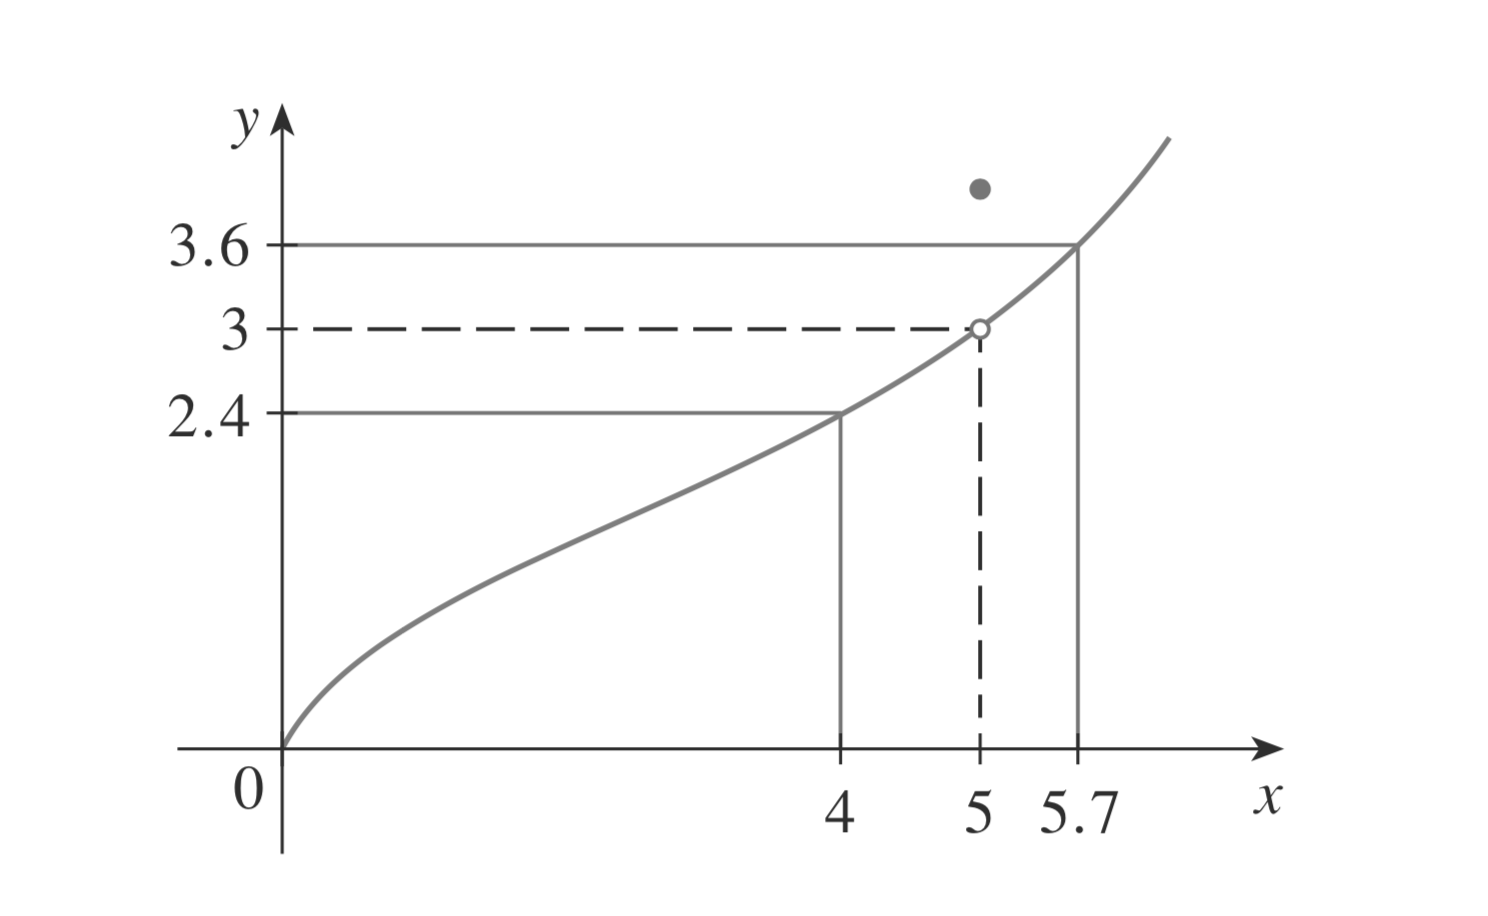
\includegraphics[width=9cm]{Function-limit-eg.png}
\caption{Plot of $y=f(x)$.}
\end{figure}
\begin{itemize}
\item What is $\lim_{x\rightarrow 5^{-}}f(x)$ ?
\item What is $\lim_{x\rightarrow 5^{+}}f(x)$ ?
\item What is $\lim_{x\rightarrow 5}f(x)$ ?
\end{itemize}
\end{frame}

\begin{frame}
\frametitle{Infinite Limit/Limit at Infinity}
\begin{itemize}
\item How to define $\lim_{x \rightarrow a}f(x) = \infty$ for $-\infty < a < +\infty$ ?
\vspace*{1.5in}
\item How to define $\lim_{x \rightarrow \infty}f(x) = a$ for $-\infty < a < +\infty$ ?
\vspace*{1.5in}
\end{itemize}
\end{frame}

\begin{frame}
\frametitle{Infinite Limit/Limit at Infinity}
\begin{itemize}
\item How to define $\lim_{x \rightarrow a}f(x) = \infty$ for $-\infty < a < +\infty$ ?

\vspace*{0.1in}
For any $M > 0$, there exists $\delta > 0$ such that
$$
f(x) > M \text{ whenever } 
0 < \vert x-a \vert < \delta.
$$
(The value of $f(x)$ approaches $\infty$ when $x$ approaches $a$.)
\vspace*{0.2in}
\item How to define $\lim_{x \rightarrow \infty}f(x) = a$ for $-\infty < a < +\infty$ ?

\vspace*{0.1in}
For any $\epsilon > 0$, there exists a $M > 0$ such that
$$
\vert f(x)-a \vert < \epsilon \text{ whenever } 
x > M.
$$
(The value of $f(x)$ approaches $a$ when $x$ approaches $\infty$.)
\vspace*{0.2in}
\end{itemize}
\end{frame}

%------------------------------------------------
%\subsection{Continuity}
\begin{frame}
\frametitle{Continuity}
A function $f$ is continuous at a number $a$ if
$$
\lim_{x \rightarrow a} f(x) = f(a).
$$
It implies 3 things:
\begin{enumerate}
\item $f(a)$ is defined ($a \in X$);
\item $\lim_{x \rightarrow a} f(x)$ exists;
\item $\lim_{x \rightarrow a} f(x) = f(a)$.
\end{enumerate}
\vspace*{0.15in}
\textbf{Right continuous}: $\lim_{x \rightarrow a^{-}} f(x) = f(a)$.
\\~\\
\textbf{Left continuous}: $\lim_{x \rightarrow a^{+}} f(x) = f(a)$.

\end{frame}

\begin{frame}
\frametitle{Continuity: Examples}
\begin{columns}[t] % The "c" option specifies centered vertical alignment while the "t" option is used for top vertical alignment

\column{.47\textwidth} % Left column and width
\vspace*{-0.15in}
\begin{figure}[H]
\centering
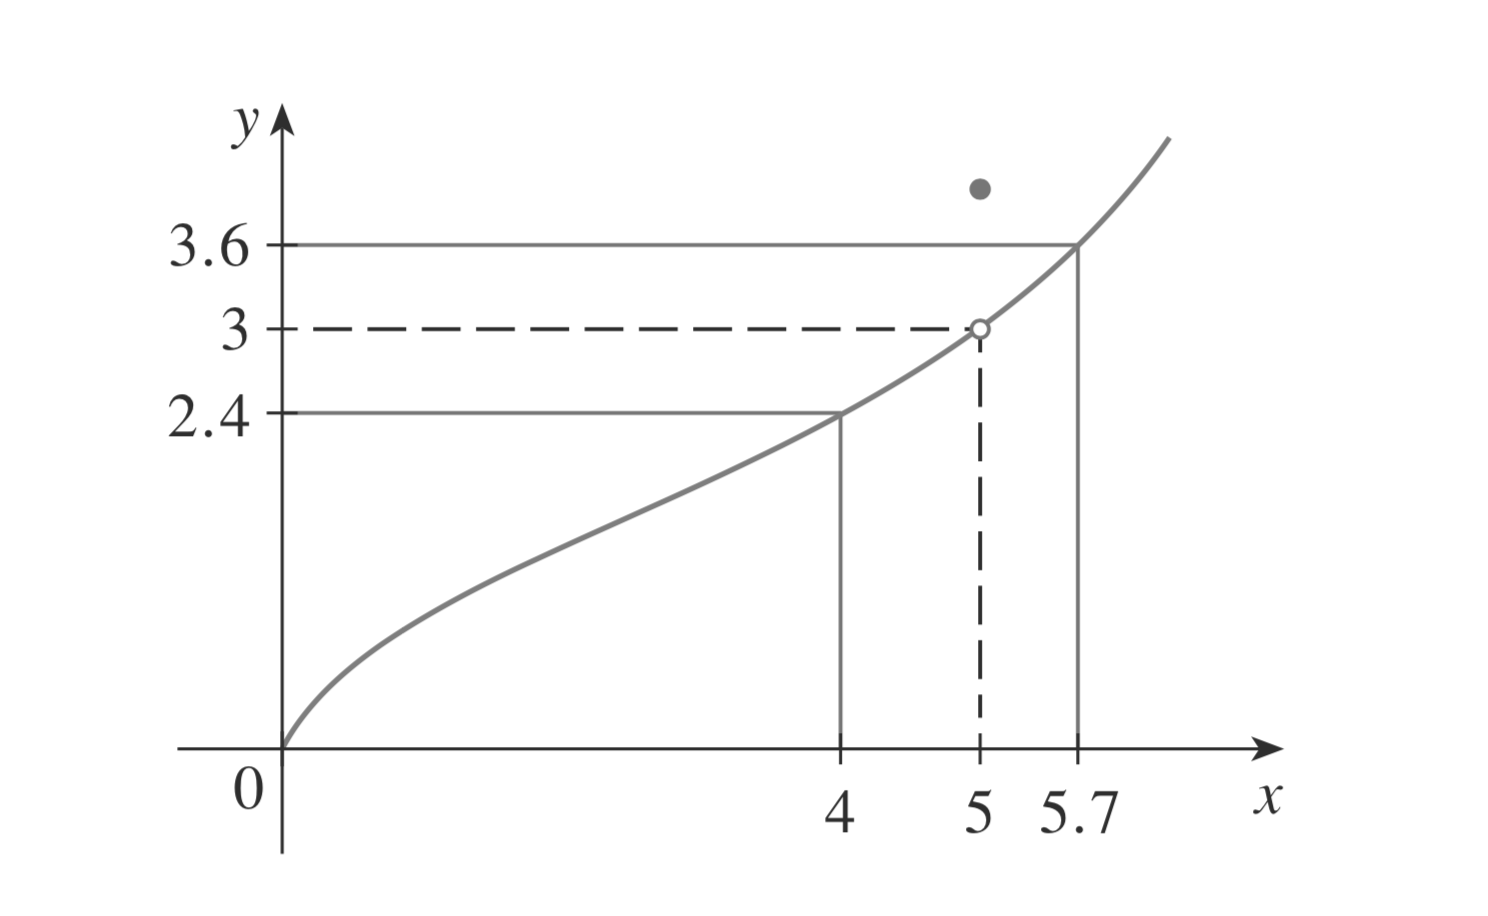
\includegraphics[width=6.2cm]{Function-limit-eg.png}
%\caption{Plot of $y=f(x)$.}
\end{figure}
This function is discontinuous at $x=5$.

\column{.47\textwidth} % Right column and width
\vspace*{-0.15in}
\begin{figure}[H]
\centering
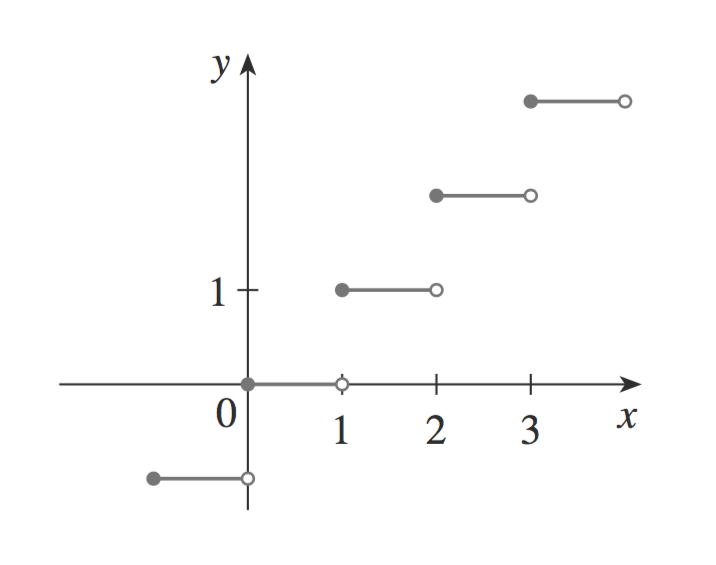
\includegraphics[width=5.5cm]{Function-cont-eg.png}
%\caption{Plot of $y=f(x)$.}
\end{figure}
\vspace*{-0.1in}
This function is discontinuous (but right continuous) at any integer $x$.

\end{columns}
 \end{frame}

% \begin{frame}
% \frametitle{Other Useful Continuity Notions}
% \begin{itemize}
% \item \textbf{Uniform continuity}: \\
% For all $\epsilon > 0$ there exists a $\delta > 0$ such that for any $x,y\in X$ with $\vert x-y \vert < \delta$ we have $\vert f(x)-f(y)\vert < \epsilon$.\\
% (A global property rather than a local one: as long as $x,y$ are sufficiently close, we can guarantee that $f(x),f(y)$ are close.)
% \vspace*{0.15in}
% \item \textbf{Lipschitz continuity}: \\
% There exists a constant $L$ such that for any $x,y\in X$, we have $\vert f(x)-f(y)\vert \leq L \vert x-y \vert$.
% \end{itemize}

% \end{frame}

% \begin{frame}
% \frametitle{Continuity: Exercise}
% Which statement(s) of the following is incorrect?
% \begin{itemize}
% \item[A] $f(x) = x^2$, $x\in \mathbb{R}$ is not uniformly continuous, but $f(x) = x^2$, $x\in [0,245]$ is Lipschitz continuous;
% \item[B] $f(x) = x^{1/3}$, $x \in [0,1]$ is Lipschitz continuous;
% \item[C] $f(x) = x^{3/2}\sin (\frac{1}{x})$ ($x\neq 0$), $f(0)=0$, $x\in [0,1]$ is uniformly continuous as well as Lipschitz continuous; 
% \item[D] Every continuous function defined on $[-1,1]$ is uniformly continuous;
% \item[E] A continuous function $f$ is defined on $[-5,5]$ and satisfies $f(-2) = -3, f(1) = 4$, then there must exist a number $x_0 \in [-2,1]$ such that $f(x_0)=0$.
% \end{itemize}
% % Answer: B C \\
% % Choice E: ``Intermediate Value Theorem''.
% \end{frame}

%------------------------------------------------
\section{Derivative}
%------------------------------------------------
\subsection{Definition and Differentiation Rules}
\begin{frame}
\frametitle{Definition of Derivative}
The derivative of function $f$ at $a\in X$, denoted by $f'(a)$ is
$$
f'(a) = \lim_{h \rightarrow 0} \frac{f(a+h)-f(a)}{h}
$$
if this limit exists (``differentiable'').
\vspace*{-0.1in}
\begin{figure}[H]
\centering
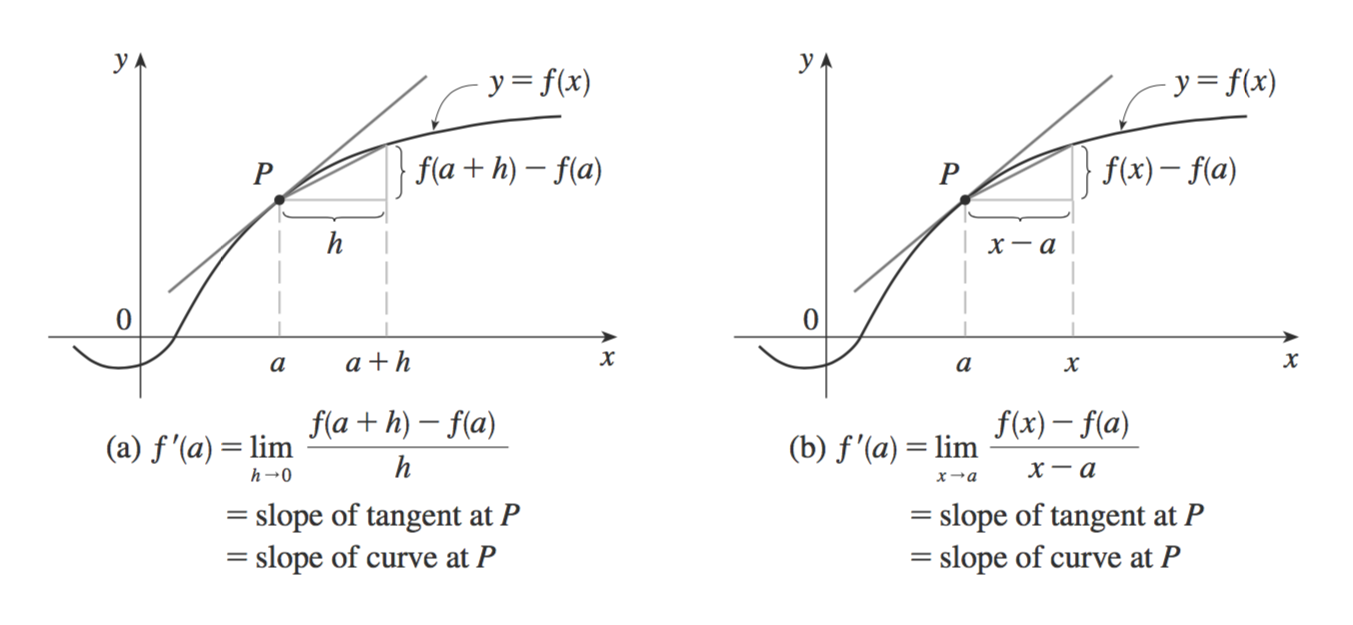
\includegraphics[width=11cm]{Derivative.png}
\vspace*{-0.15in}
\caption{Geometric interpretations of the derivative.}
\end{figure}

\end{frame}

\begin{frame}
\frametitle{Differentiation Rules}
Derivatives of some common functions:
\begin{itemize}
\item $f(x)=const$, then $f'(x)=0$;
\item $f(x) = x^{\alpha}, \alpha \neq 0$, then $f'(x) = \alpha x^{\alpha-1}$;
\item $(e^{x})'= e^{x}$, $(\ln x)' = 1/x$ ($x > 0$);
\item $(\sin x)' = \cos x$, $(\cos x)' = -\sin x$, $(\tan x)' = 1/\cos ^2 x$;
\item $(\sin^{-1} x)' = 1/\sqrt{1-x^2}$, $(\cos^{-1} x)' = -1/\sqrt{1-x^2}$, $(\tan^{-1} x)' = 1/{1+x^2}$.
\end{itemize}
If both $f(x)$ and $g(x)$ are differentiable:
\begin{itemize}
\item $(cf(x))' = cf'(x)$, $(f(x)+g(x))' = f'(x)+g'(x)$;
\item $(f(x)g(x))' = f'(x)g(x) + f(x)g'(x)$;
\item  $\left(\frac{f(x)}{g(x)} \right)'=\frac{f'(x)g(x) - f(x)g'(x)}{g^2(x)}$ (assume $g(x) > 0$);
\item The \textbf{chain rule}: if $F = f \circ g$, then $F'(x) = f'(g(x))g'(x)$.
\end{itemize}
\end{frame}

\begin{frame}
\frametitle{Derivative: Exercises}
\begin{columns}[t] % The "c" option specifies centered vertical alignment while the "t" option is used for top vertical alignment

\column{.47\textwidth} % Left column and width
1. Find the derivatives of the following functions
\begin{itemize}
\item $f(x) = x e^x$;
\item $f(x) = 1 - \cos^2 x$;
\item $f(x) = \frac{\ln x}{x}$.
\end{itemize}

\column{.47\textwidth} % Right column and width
% 2. $f(x) = \frac{1}{\sqrt{\gamma}} \exp \left(-\frac{(x-\mu)^2}{\gamma}\right)$ where constants $\gamma > 0$ and $\mu \in \mathbb{R}$, and $x\in \mathbb{R}$. Calculate $f'(x)$ and find $x_0 \in \mathbb{R}$ such that the tangent line of $f(x)$ at $x_0$ is horizontal.
%\\~\\
2. Find $\lim_{x \rightarrow 0} (1+x)^{1/x}$.

\end{columns}
\end{frame}

\begin{frame}
\frametitle{Solution to Exercise 2}
Let $f(x) = \ln x$, then
\begin{equation*}
\begin{aligned}
f'(1) &= \lim_{x \rightarrow 0} \frac{\ln (1+x) - \ln 1}{x} \\
&= \lim_{x \rightarrow 0} \frac{1}{x} \ln (1+x) \\
&= \lim_{x \rightarrow 0} \ln (1+x)^{1/x}.
\end{aligned}
\end{equation*}
Since $f'(1)=1$, $\lim_{x \rightarrow 0} (1+x)^{1/x} = e^{1} = e$.
\end{frame}

%------------------------------------------------

\subsection{Application of Derivatives}

\begin{frame}
\frametitle{Minimum and Maximum}
\begin{theorem}[Fermat's Theorem]
If $f$ has a local minimum or maximum at $c$ and $f'(c)$ exists, then $f'(c)=0$.
\end{theorem}
\textbf{Note}: the converse is not true.
\vspace*{0.15in}
\begin{theorem}[The Second Derivative Test]
If $f$ has second derivative on $(c-\epsilon_0,c+\epsilon_0)$ for a certain $\epsilon_0 > 0$, then
\begin{itemize}
\item if $f'(c)=$ and $f'(c) > 0$, $f$ has a local minimum at $c$;
\item if $f'(c)=$ and $f'(c) < 0$, $f$ has a local maximum at $c$.
\end{itemize}
\end{theorem}
\end{frame}

\begin{frame}
\frametitle{Minimum and Maximum: Example}
Let $v_1$ be the velocity of light in air and $v_2$ the velocity of light in water. According to Fermat's Principle, a ray of light will travel from a point $A$ in the air to a point $B$ in the water by a path $ACB$ that \textbf{minimizes} the time taken. Then
$$
\frac{\sin \theta_1}{\sin \theta_2} = \frac{v_1}{v_2},
$$
where $\theta_1$ is the angle of incidence and $\theta_2$ is the angle of refraction. This equation is known as \textbf{Snell's Law}.
\begin{figure}
\centering
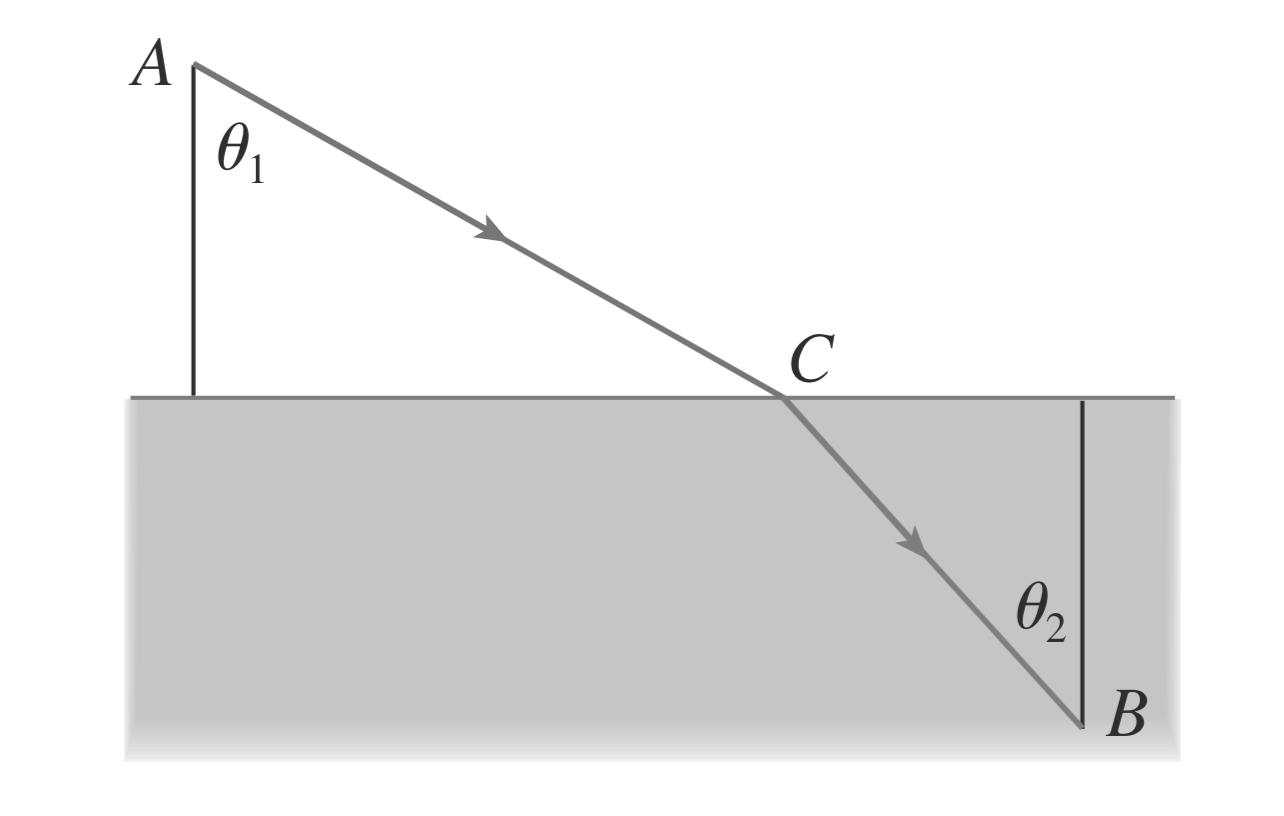
\includegraphics[width=5.5cm]{Snells-Law.png}
\end{figure}

\end{frame}

\begin{frame}
\frametitle{Convexity}
A function defined on a convex set $X$, $f: X \rightarrow \mathbb{R}$ is convex if for any $x,y \in X$ and $t \in [0,1]$, 
$$
f(tx+(1-t)y) \leq tf(x) + (1-t)f(y).
$$
Visually, a convex function has a ``curve up'' shape:
\begin{figure}
\centering
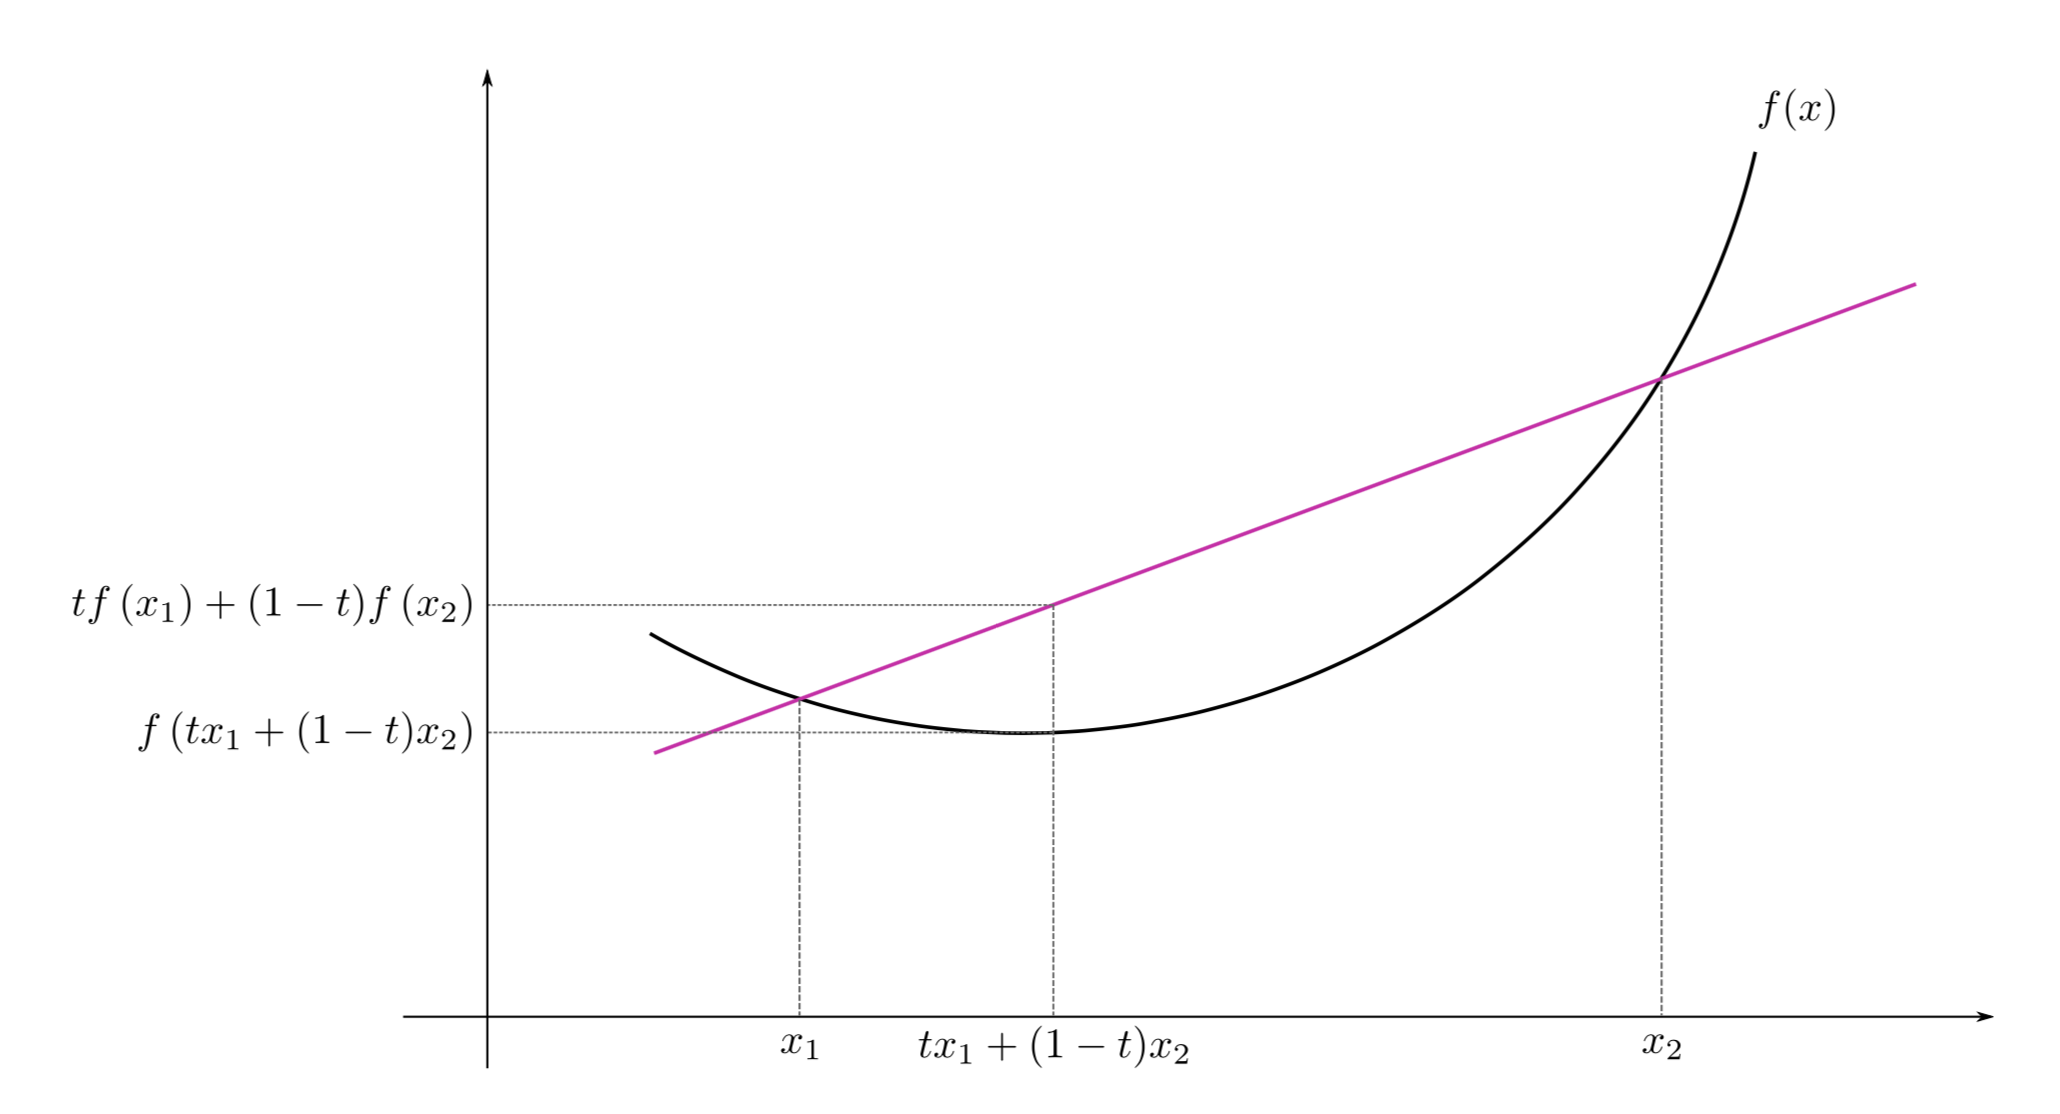
\includegraphics[width=8cm]{Convex-Function.png}
\end{figure}

\end{frame}

\begin{frame}
\frametitle{Convexity and Derivatives}
Suppose $f(x)$ is twice differentiable on interval $I$, then
\begin{itemize}
\item $f$ is convex on $I$ if and only if $f'(x)$ is monotonically non-decreasing on $I$;
\item $f$ is convex on $I$ if and only if $f''(x) \geq 0$ for $x \in I$  (often used to test for convexity).
\end{itemize}
~\\
A nice property of convexity:\\
Any local minimum of a convex function is also a global minimum; a strictly convex function has at most one global minimum. (Therefore convexity is much desired in optimization.)

\end{frame}

\begin{frame}
\frametitle{Review Exercises: Morning Session}
\begin{columns}[t] % The "c" option specifies centered vertical alignment while the "t" option is used for top vertical alignment

\column{.47\textwidth} % Left column and width
% 1. Are all Lipschitz continuous functions defined on $[-1,1]$ also differentiable on $(-1,1)$? If not, give a counterexample.
% \\~\\
1. Calculate $\lim_{x \rightarrow 0} \frac{\sin x}{x}$ and $\lim_{x \rightarrow 0} \frac{\tan x}{x}$.
% (hint: use the definition of derivatives)
\\~\\
2. Which following functions are convex?
\begin{itemize}
\item[A] $f_1(x) = \vert x \vert, x\in [-1,1]$;
\item[B] $f_2(x) = \ln(x^2+1), x \in \mathbb{R}$;
\item[C] $f_3(x) = e^{-x}, x\in \mathbb{R}$.
\end{itemize}
% answer: A C

\column{.47\textwidth} % Right column and width
3. Let $f(x) = \frac{1}{x}, x>0$. For every positive integer $n$, find $f^{(n)}(x)$.
\\~\\
4. $f(x) = \frac{1}{\sqrt{\gamma}} \exp \left(-\frac{(x-\mu)^2}{\gamma^2}\right)$ where constants $\gamma > 0$ and $\mu \in \mathbb{R}$, and $x\in \mathbb{R}$. Find all the global maximums of $f(x)$.

\end{columns}
\end{frame}

\begin{frame}
\frametitle{Taylor Expansion}

\href{https://youtu.be/3d6DsjIBzJ4}{\textbf{Talor Series}, by \textit{3Blue1Brown}}
\end{frame}

\begin{frame}
\frametitle{Challenge Exercises: Morning Session}
\begin{columns}[t] % The "c" option specifies centered vertical alignment while the "t" option is used for top vertical alignment

\column{.47\textwidth} % Left column and width
1. Find the Taylor expansion of $f(x) = \tan x$ around $0$ and use the result to show that $\lim_{x \rightarrow 0} \frac{\tan x}{x} = 1$.
\\~\\
2. Calculate $\sum_{x=0}^{\infty} \frac{e^{-\lambda}\lambda^x}{x!}$. Here $\lambda > 0$ is a constant and $x \in \mathbb{N}$. ($0!=1$.)
% Use the Taylor expansion of $f(x) = e^x$ around $0$.
\\~\\
3. Let $f(x) = x^{\alpha - 1}(1-x)^{\beta-1}, x\in (0,1)$, where $\alpha, \beta > 0$ are constants. Find all the minimums and maximums (if there are any) of $f$.

\column{.47\textwidth} % Right column and width
% 4. $f(x)$ is a convex function on $\mathbb{R}$, $P = (x_0,f(x_0))$ is a point on $f(x)$, and $l$ is the tangent line of the curve of $f(x)$ at $P$. Choose the correct statement(s).
% \begin{itemize}
% \item[A] $l$ must lie above or on the curve of $f(x)$;
% \item[B] $l$ must lie below or on the curve of $f(x)$;
% \item[C] $l$ can intersect with $f(x)$ at multiple points.
% \end{itemize}
4. The following figure shows the graphs of $f$, $f'$, $f''$, and $f'''$. Identify each curve.
\vspace*{-0.2in}
\begin{figure}[H]
\centering
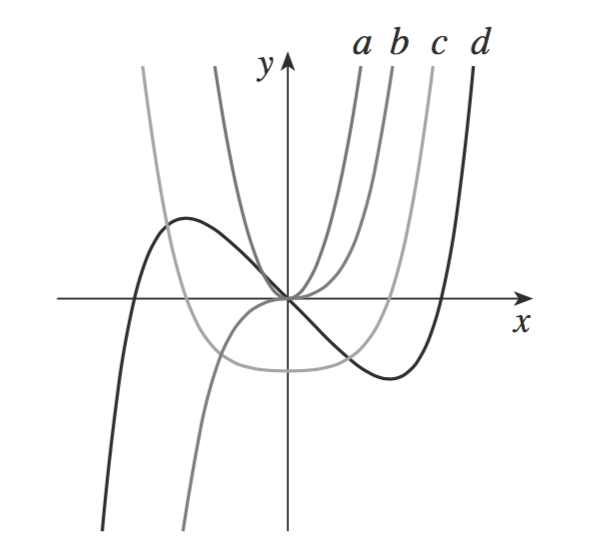
\includegraphics[width=5.5cm]{Derivative-ex-1.png}
\end{figure}
% Answer: d,c,b,a

\end{columns}
\end{frame}

%------------------------------------------------

\section{Integrals}
\subsection{Definite Integrals}
\begin{frame}
\frametitle{Properties of Definite Integrals}
Let $a \leq d \leq b \in \mathbb{R}$:
\begin{itemize}
\item If $c \in \mathbb{R}$ is a constant, then $\int_{a}^b c dx = c(b-a)$;
\item $\int_{a}^b cf(x) dx = c\int_{a}^b f(x) dx$;
\item $\int_{a}^b [f(x)+g(x)] dx = \int_{a}^b f(x) dx + \int_{a}^b g(x) dx$;
\item $\int_{a}^d f(x) dx + \int_{d}^b f(x) dx = \int_{a}^b f(x) dx$;
\item If $f(x) \geq g(x)$ for $a \leq x \leq b$, then $\int_{a}^b f(x) dx \geq \int_{a}^b g(x) dx$;
\item If $m \leq f(x) \leq M$ for $a \leq x \leq b$, then $m(b-a) \leq \int_{a}^b f(x) dx \leq M(b-a)$.
\end{itemize}
\end{frame}

\begin{frame}
\frametitle{The Fundamental Theorem of Calculus}
If $f$ is continuous on $[a,b]$, then:
\begin{itemize}
\item function $g(x) = \int_a^x f(x) dx, a\leq x \leq b$ is continuous on $[a,b]$ and differentiable on $(a,b)$, and $g'(x) = f(x)$;
\item $\int_a^b f(x)dx = F(b)-F(a)$, where $F$ is any anti-derivative of $f$ ($F' = f$).
\end{itemize}
\vspace*{0.15in}
A mini-exercise: 
find $\frac{d}{dx}\int_1^x \sin x^4 dx$.

\end{frame}

\begin{frame}
\frametitle{Useful Rules for Integration}
\begin{itemize}
\item \textbf{Substitution rule}: If $u=g(x)$ is continuously differentiable on $[a,b]$ and $f$ is continuous on the range of $u$, then 
$$
\int_a^b f(g(x))g'(x)dx = \int_{g(a)}^{g(b)} f(u)du.
$$ 
\item \textbf{Integration by parts}: If functions $u$ and $v$ are both continuously differentiable on $[a,b]$, then
$$
\int_{a}^{b} u(x)v'(x)dx = \left .[u(x)v(x)] \right\vert_{a}^{b} - \int_{a}^{b} v(x)u'(x)dx.
$$
\end{itemize}
\end{frame}

\begin{frame}
\frametitle{Integration: Exercises}
\begin{enumerate}
\item Calculate $\int_{1}^e \frac{\ln x}{x} dx$.
\vspace*{1.2in}
\item Calculate $\int_{0}^1 x \cos x dx$.
\vspace*{1.2in}
\end{enumerate}
\end{frame}

\subsection{Improper Integrals}
\begin{frame}
\frametitle{Improper Integrals}
\begin{enumerate}
\item \textbf{Infinite intervals}: if $\int_{a}^{t}f(x)dx$ exists for every $t\geq a$ then 
$$
\int_{a}^{\infty}f(x)dx = \lim_{t \rightarrow \infty}\int_{a}^{t}f(x)dx
$$ 
provided that this limit exists (convergent); similarly, one may define $\int_{-\infty}^{a}f(x)dx$, and if both $\int_{a}^{\infty}f(x)dx$ and $\int_{-\infty}^{a}f(x)dx$ are convergent, then $\int_{-\infty}^{\infty}f(x)dx = \int_{-\infty}^{a}f(x)dx + \int_{a}^{\infty}f(x)dx$.
\item \textbf{Discontinuous integrand}: if $f$ is continuous on $[a,b)$ and is discontinuous at $b$, then
$$
\int_a^b f(x) dx = \lim_{t \rightarrow b^-} \int_a^t f(x)dx
$$
if this limit exists; similarly, if $f$ is continuous on $(a,b]$ and is discontinuous at $a$, $\int_a^b f(x) dx = \lim_{t \rightarrow a^+} \int_t^b f(x)dx$.
\end{enumerate}
\end{frame}

\begin{frame}
\frametitle{Improper Integrals: Exercises}
\begin{enumerate}
\item For what values of $p \in \mathbb{R}$ is the integral
$$
\int_1^{\infty} \frac{1}{x^p} dx
$$
convergent?
% answer: convergent if $p>1$ and divergent if $p \leq 1$.
\vspace*{1in}
\item Evaluate $\int_2^5 \frac{1}{\sqrt{x-2}} dx$.
% answer: 2\sqrt{3}.
\vspace*{1.2in}
\end{enumerate}
\end{frame}

%------------------------------------------------

\section{Sequences and Series}
\begin{frame}
\frametitle{Basics of Sequences}
A \textbf{sequence }is a list of numbers written in a definite order. We often denote a sequence $\{a_1,a_2,a_3,\ldots\}$ by $\{a_n\}$ or $\{a_n\}_{n=1}^{\infty}$.
\\~\\
A sequence $\{a_n\}$ has \textbf{limit} $L$ (written as $\lim_{n \rightarrow \infty} a_n = L$, or $a_n \rightarrow L$ as $n\rightarrow \infty$) if for every $\epsilon > 0$ there is a corresponding integer $N$ such that $\vert a_n - L \vert < \epsilon$ whenever $n > N$.
\\~\\
If for every $n \in \mathbb{N}$, $a_n \leq a_{n+1}$ (increasing) or $a_n \geq a_{n+1}$ (decreasing), then the sequence $\{a_n\}$ is \textbf{monotonic}. If there exists a number $M > 0$ such that $\vert a_n \vert \leq M$ for every $n$ then the sequence $\{a_n\}$ is \textbf{bounded}.
\\~\\
\textbf{Monotonic Sequence Theorem:} Every bounded, monotonic sequence is convergent (has a limit).
\end{frame}

\begin{frame}
\frametitle{Sequences: Exercises}
\begin{enumerate}
\item Find the limit of the sequence ${a_n}$ where $a_n = \left(1+\frac{1}{n}\right)^n$, $n \in \mathbb{N}$.
\vspace*{1.2in}
\item Let $a_n = \frac{2^n}{n!}$, $n \in \mathbb{N}$. Is the sequence ${a_n}$ convergent? If so, what is its limit?
\vspace*{1.2in}
\end{enumerate}
\end{frame}

\begin{frame}
\frametitle{Basics of Series}
A \textbf{series} can be thought of as the infinite sum of a sequence ${a_n}$, written as $\sum_{n=1}^{\infty} a_n$ or $\sum a_n$. More formally, it can be defined by taking the limit of partial sums $\{s_n\}$, where $s_n = \sum_{i=1}^{n} a_i$: if $\lim_{n \rightarrow \infty} s_n$ exists then the series $\sum a_n$ is convergent, otherwise it is divergent.
\\~\\
If $\sum_{n=1}^{\infty} a_n$ is convergent, then $\lim_{n \rightarrow \infty} a_n = 0$.
\\~\\
An important example - \textbf{the geometric series}:\\
$$
\sum_{n=1}^{\infty} ar^{n-1} = a + ar + ar^2 + \cdots
$$
is convergent if $\vert r \vert < 1$ and its sum is 
$\sum_{n=1}^{\infty} ar^{n-1} = \frac{a}{1-r}$.
If $\vert r \vert \geq 1$, the geometric series is divergent.
\end{frame}

\begin{frame}
\frametitle{Series: Exercises}
\begin{enumerate}
\item Show that $\sum_{n=1}^{\infty} \frac{1}{n(n+1)}$ is convergent and find its sum.
% answer: 1; simplify the expression of the partial sum and take the limit.
\vspace*{1.2in}
\item Find $\sum_{n=0}^{\infty} x^n$ where $\vert x \vert < 1$.
% answer: $\frac{1}{1-x}$.
\vspace*{1.2in}
\end{enumerate}
\end{frame}

\begin{frame}
\frametitle{Convergence of Series}
Commonly used tests for convergence:
\begin{enumerate}
\item \textbf{The comparison test}: Suppose that $\sum a_n$ and $\sum b_n$ are series with positive terms. 
\begin{itemize}
\item[(i)] If $\sum b_n$ is convergent and $a_n \leq b_n$ for all $n$, then $\sum a_n$ is also convergent;
\item[(ii)] If $\sum b_n$ is divergent and $a_n \geq b_n$ for all $n$, then $\sum a_n$ is also divergent.
\item Video example: \href{https://youtu.be/4yyLfrsSXQQ}{\textbf{famous proof that the harmonic series diverges}, by \textit{Khan Academy}}.
\end{itemize}
%\item \textbf{The limit comparison test}: Suppose that $\sum a_n$ and $\sum b_n$ are series with positive terms. If $\lim_{n \rightarrow \infty} \frac{a_n}{b_n} = c$ where $c$ is a finite positive number, then either both series converge or both diverge.
\item \href{https://youtu.be/xRyXz_UZ14Q}{\textbf{The integral test} (by \textit{Khan Academy})}.
\item \textbf{The alternating series test}: If the alternating series $\sum_{n=1}^{\infty} (-1)^{n-1} b_n$ ($b_n > 0$) satisfies (i) $b_{n+1} \leq b_n$ for all $n$, and (ii) $\lim_{n \rightarrow \infty} b_n = 0$ then the series is convergent.
\end{enumerate}
\end{frame}

\begin{frame}
\frametitle{Review Exercises: Afternoon Session}
\begin{columns}[t] % The "c" option specifies centered vertical alignment while the "t" option is used for top vertical alignment

\column{.47\textwidth} % Left column and width
1. Evaluate the following definite integrals:
\begin{itemize}
\item $\int_0^4 \frac{x}{\sqrt{x^2+9}}dx$;
% answer: $2$
%\item $\int_0^1 \frac{2x}{1+x^4} dx$.
% answer: $\pi/4$
%\end{itemize}
%~\\
%2. Evaluate the following definite integrals:
%begin{itemize}
\item $\int_0^1 x\ln xdx$;
% answer: $-1/4$
%\item $\int_0^{\pi} e^x\sin xdx$.
%% answer: $(e^{\pi}+1)/2$
\end{itemize}
~\\
2. If $f$ is continuous on $\mathbb{R}$, show that
$$
\int_{a}^{b} f(x+c) dx = \int_{a+c}^{b+c} f(x) dx.
$$

\column{.47\textwidth} % Right column and width
3. Do the following series converge? Calculate the value of the infinite sum for each convergent series.\\
(a) $\sum_{n=2}^{\infty} 5^{n-1}\left(\frac{9}{10}\right)^{n}$;\\
(b) $\sum_{n=1}^{\infty} \left(\frac{3}{2}\right)^{n}\frac{1}{9^{n+2}}$.
\\~\\
4. True or false?
\begin{itemize}
\item If $x_n \rightarrow 0$ as $n \rightarrow \infty$, then $\sum_{n=1}^{\infty} x_n$ is convergent;
\item $\sum_{n=1}^{\infty} x^n e^{-nx}$ is convergent for any $x > 0$;
\item $\sum_{n=2}^{\infty} \frac{1}{n \ln n}$ is convergent.
\end{itemize}
% answer: F T F
\end{columns}
\end{frame}

%------------------------------------------------
\section{Multivariate Calculus}

\begin{frame} 
\frametitle{Partial Derivatives}
If $u$ is a function of $n$ variables, $u = f(x_1,x_2,\ldots,x_n)$, its partial derivative with respect to the $i$th variable $x_i$ is
$$
\frac{\partial u}{\partial x_i} = \lim_{h \rightarrow 0} \frac{f(x_1,\ldots,x_{i-1},x_i+h,x_{i+1},\ldots,x_n)-f(x_1,\ldots,x_i,\ldots,x_n)}{h}.
$$
(Strategy: treat all the other variables as constants and take the derivative with respect to the variable of interest.)
\\~\\
Suppose $u = f(x_1,x_2,\ldots,x_n)$ is defined on $\mathbb{R}^n$. If $\frac{\partial^2 u}{\partial x_i\partial x_j}$ and $\frac{\partial^2 u}{\partial x_j\partial x_i}$ are both continuous on $\mathbb{R}^n$, then $\frac{\partial^2 u}{\partial x_i\partial x_j} = \frac{\partial^2 u}{\partial x_j\partial x_i}$.
\end{frame}

\begin{frame} 
\frametitle{The Gradient Vector and Hessian Matrix}
Suppose $f(x_1,x_2,\ldots,x_n)$ is a function of $n$ variables such that all the partial derivatives exist, then the gradient vector of $f$ is
$$
\nabla f = \left(\frac{\partial f}{\partial x_1},\frac{\partial f}{\partial x_2}, \ldots,\frac{\partial f}{\partial x_n}\right).
$$
If all the second-order partial derivatives of $f$ also exist, the Hessian matrix of $f$ is
$$
H = 
\begin{bmatrix}
    \frac{\partial^2 f}{\partial x_1^2} & \frac{\partial^2 f}{\partial x_1\partial x_2} &  \dots  & \frac{\partial^2 f}{\partial x_1\partial x_n} \\
    \frac{\partial^2 f}{\partial x_2\partial x_1} & \frac{\partial^2 f}{\partial x_2^2} &  \dots  & \frac{\partial^2 f}{\partial x_2\partial x_n}\\
    \vdots & \vdots &  \ddots & \vdots \\
    \frac{\partial^2 f}{\partial x_n\partial x_1} & \frac{\partial^2 f}{\partial x_n\partial x_2} &  \dots  & \frac{\partial^2 f}{\partial x_n^2}
\end{bmatrix}.
$$
\end{frame}

\begin{frame} 
\frametitle{Change of Variables}
Take the two-variable case as an example:\\
Suppose $z=f(x,y)$ is function of $x,y$ and $x = u(s,t)$, $y = v(s,t)$ with respect two other variables $s,t$, then $z=g(s,t)$ as a function of $s,t$, where
$$
g(s,t) = f(u(s,t),v(s,t))\vert J\vert.
$$
Here $J$ is the \textbf{Jacobian} of the transformation $x = u(s,t)$, $y = v(s,t)$:
$$
J =
\begin{vmatrix}
\frac{\partial x}{\partial s} & \frac{\partial x}{\partial t} \\
\frac{\partial y}{\partial s} & \frac{\partial y}{\partial t}
\end{vmatrix}
= \frac{\partial x}{\partial s}\frac{\partial y}{\partial t} - \frac{\partial x}{\partial t}\frac{\partial y}{\partial s}.
$$
~\\
Suppose that we want to integrate $f(x,y)$ over a region $R$. Under the transformation $x = u(s,t)$, $y = v(s,t)$ the regions becomes $S$ and the integral becomes:
$$
\iint_R f(x,y) dxdy = \iint_S f(u(s,t),v(s,t))\vert J\vert dsdt.
$$
\end{frame}
% \begin{frame} 
% \frametitle{Integration: Fubini Theorem}

% \end{frame}

\begin{frame}
\frametitle{Multivariate Calculus Review Exercises}
\begin{enumerate}
\item Let $f(x,y,z)=ye^x \ln z + z \tan z$ ($z \in (0,\frac{\pi}{2})$) and $g(x,y,z)=x^3y+y^3z+z^5+\sqrt{xy}z$.\\ Compute $\frac{\partial f}{\partial y}$, $\frac{\partial f}{\partial z}$, $\frac{\partial g}{\partial x}$, and $\frac{\partial g}{\partial y}$.
%\\~\\ answer: $e^x \ln z$, $\frac{ye^x}{z}+\tan z + \frac{z}{\cos^2 z}$, $3x^2y + \frac{\sqrt{y}z}{2\sqrt{x}}$, and $x^3 + 3y^2 z + \frac{\sqrt{x}z}{2\sqrt{y}}$.
\vspace*{0.5in}
\item $f(x,y) = \frac{1}{\sqrt{2\pi y^2}}e^{-\frac{(x-s)^2}{2y^2}}$, where $s \in \mathbb{R}$ is a constant. Obtain the gradient vector and Hessian matrix of $f$.
\vspace*{0.5in}
\item Evaluate the double integral $\int_1^3 \int_0^2 (xy + x^2y^3)dydx$.
\end{enumerate}



%\\~\\ answer: $42\frac{2}{3}$

\end{frame}

%------------------------------------------------
\begin{frame}
\frametitle{Challenge Exercises: Afternoon Session}
\begin{columns}[t] % The "c" option specifies centered vertical alignment while the "t" option is used for top vertical alignment

\column{.47\textwidth} % Left column and width
1. Given that $\int_1^{\infty} \frac{1}{x} dx = \infty$ and $\sum_{n=1}^{\infty} \frac{1}{n} = \infty$, use two methods to show that $\sum_{n=1}^{\infty} \frac{1}{n^p} = \infty$ for any $p \in (0,1)$.
\\~\\
%2. Find $\lim_{x\rightarrow 3} \frac{x}{x-3} \int_{3}^{x} \frac{\sin t}{t} dt$.
2. Evaluate the following definite integrals:
\begin{itemize}
\item $\int_0^1 \frac{2x}{1+x^4} dx$.
% answer: $\pi/4$
\item $\int_0^{\pi} e^x\sin xdx$.
% answer: $(e^{\pi}+1)/2$
\end{itemize}
%~\\
\column{.47\textwidth} % Right column and width
3. The Gamma function $\Gamma (x)$ is defined for any real number $x > 0$ as $\Gamma (x) = \int_{0}^{\infty} t^{x-1}e^{-t}dt$. Show that $\Gamma (x+1) = x\Gamma (x)$.
% Use integration by parts.
\\~\\
4. Evaluate $\int_{0}^{\infty} e^{x^2} dx$.\\
(Hint: start with $\int_{0}^{\infty}\int_{0}^{\infty} e^{x^2+y^2} dxdy$.)
%\\~\\
\end{columns}

\end{frame}


%------------------------------------------------

% \begin{frame}
% \Huge{\centerline{The End}}
% \end{frame}

%----------------------------------------------------------------------------------------

\end{document}